\chapter{Introdução} 
\label{cap:introducao}


Os manipuladores robóticos já fazem parte do cotidiano em vários processos de
produção industrial. Em se tratando de robótica móvel, a sua aplicação prática
ainda apresenta muitos desafios. Na robótica móvel, a navegação é a capacidade
do veículo de se locomover no ambiente, podendo ser guiada (tele operada),
autônoma ou híbrida (semiautônoma). A navegação autônoma é totalmente dependente
do aparato sensorial acessível ao robô, pois a percepção e estímulos do ambiente
precisam ser capturados para que este possa reagir de acordo. As características
físicas do robô também vão limitar seu comportamento em relação a sua mobilidade
(restrições cinemáticas), onde o aparato sensorial e motor também devem ser
propícios para a execução de suas tarefas. A capacidade de se deslocar de forma
autônoma e segura depende certamente de um determinado grau de “inteligência” do
dispositivo de controle e navegação do robô. Através do uso de técnicas de
Inteligência Artificial se busca traduzir em algoritmos estes processos de
controle e navegação inteligente.

A capacidade de locomoção é própria dos animais. Em robôs móveis, para mimetizar
essa capacidade, dotam-se os mesmos de aparatos motores e sensoriais, podendo
estes, ser ou não inspirados na fisiologia dos animais \cite{Webb2000}. Tais
aparatos são fundamentais e definem a capacidade, características e
especificidades dos movimentos. A visão é um subsistema biofísico sensorial que
podemos associá-la intuitivamente às especificidades e características das
estratégias de locomoção nos animais. Portanto, implementar um sistema de visão
artificial com capacidade sensorial em um robô móvel, significa dotá-lo de um
sistema análogo de percepção, que irá permitir que este realize tarefas de
movimentação e deslocamento de modo similar. Para Marr \cite{Marr1982}, a visão
é acima de tudo uma tarefa de processamento de informações, porém, como a
informação é representada a partir de imagens, o tratamento destas é um dos
principais problemas que precisa ser investigado. Desta forma, a constituição de
um sistema de visão computacional adequado para um determinado problema, como a
navegação robótica, ainda é uma tarefa desafiadora.

Apesar da inspiração biológica no tratamento de problemas computacionais ser
mais notória nos dias de hoje, apresentando-se como algo mais recente através da
difusão das áreas de estudo multidisciplinares, como a computação cognitiva,
biologia computacional, computação bio inspirada e bioinformática; o processo
indutivo de observação da natureza biológica já era notório como motivação para
os algoritmos computacionais em décadas passadas \cite{Poggio1984}.

Porém, as pesquisas nesta área não se baseiam puramente em descobertas baseadas
na observação dos sistemas naturais, a nossa capacidade de inventar traz também
a introdução de diversas novas tecnologias ao dia a dia. Da mesma maneira, a
capacidade de combinar diversas abordagens tecnológicas em aplicações práticas
permite o desenvolvimento concreto de ferramentas e utensílios que com o passar
do tempo se tornam parte do cotidiano e até indispensáveis. Aplicação mais
abrangentes e concretas dos Robôs Móveis Autônomos (RMA) ainda dependem de
muitos avanços nas pesquisas científicas e tecnológicas, mas já é possível
visualizar a sua viabilidade através da combinação de abordagens bem sucedidas
em diversas áreas para diversos tipos de aplicações junto a sociedade, tanto do
ponto de vista econômico quanto do ponto de vista das tecnologias que já estão
sendo embarcada nestes dispositivos.


% lido 2012-10-10 ok

\section{Objetivo e Motivação}
%\label{sec:motivacao}

Este trabalho tem por objetivo o desenvolvimento de um sistema de navegação
autônoma baseado em visão computacional a fim de capacitar um veículo terrestre
autônomo a se locomover em ambientes externos não estruturados, ou seja, em
campos com vegetação/plantação e/ou em florestas pouco densas. O veículo deverá
ser capaz de se dirigir até uma localização determinada, desviando dos
obstáculos de forma autônoma, e escolhendo por meios próprios o
caminho a seguir. O veículo autônomo deverá ter a capacidade de identificar os
elementos do terreno onde irá se deslocar, identificando o chão e os obstáculos,
a fim de evitar zonas não transponíveis ou muito acidentadas. Este tipo de
sistema robótico tem vasta aplicabilidade, o interesse por essas aplicações na
área da robótica móvel tem sido demonstrado tanto pelo surgimento de grupos de
pesquisa como pelas conferências e publicações na área.

Exemplo de aplicação deste tipo de sistema pode ser visto no trabalho de
\cite{Pessin2008} onde foi avaliado a utilização de veículos autônomos no
combate a incêndios florestais. Este tipo de aplicação requer que um (ou mais)
veículo se desloque de um ponto de origem (base) até um destino determinado
(foco de incêndio) utilizando coordenadas de GPS desviando de obstáculos e se
deslocando em um terreno irregular e não estruturado.

Por outro lado, a visão computacional ainda é uma área com diversos problemas em
aberto (o próprio funcionamento da visão animal ainda é pouco conhecido), sendo
uma importante fonte de informação sensorial para a robótica móvel. A informação
visual, assim como para os animais, tem forte relação com a capacidade de
localização e locomoção autônoma, sendo de grande relevância para a robótica
móvel.

%OSORIO
%Podia adicionar aqui na motivação um parágrafo que apresenta exemplos
% "concretos" de possíveis aplicações do sistema que está sendo proposto:
%- O exemplo mais direto é o tema tratado pelo Pessin (mestrado e doutorado), do
% combate a incêndios em florestas que necessitam de veículos autônomos com esta 
%capacidade de navegação entre 2 coordenadas (atual e destino) e com desvio de
%obstáculos.
%- Um exemplo mais arrojado é o dos robôs des exploração interplanetária (Marte)
% que também tem executado funções similares e que representam o estado-da-arte 
%nesta área da robótica (onde estes não são completamente autônomos!)...


%2010-10-14 REVISAR

%\section{Objetivo Geral}
\label{sec:obj_geral}

O objetivo geral deste trabalho é desenvolver um sistema de navegação autônoma baseado
em visão computacional a fim de capacitar um veículo terrestre autônomo a se locomover em
ambientes externos não estruturados, ou seja, em campos com vegetação/plantação e/ou em
florestas pouco densas. O veículo deverá ser capaz de se dirigir até uma localização determinada,
desviando dos obstáculos, percebendo-os de forma autônoma, e escolhendo por meios próprios o
caminho a seguir. O veículo autônomo deverá ter a capacidade de identificar os elementos do terreno
onde irá se deslocar, identificando o chão e os obstáculos, a fim de evitar zonas não transponíveis ou
muito acidentadas. Portanto, o objetivo deste trabalho é desenvolver um sistema de navegação
robusto e seguro voltado à aplicação em veículos autônomos para ambientes externos não
estruturados (ou muito pouco estruturados), baseado no uso de visão computacional realizada
através da captura de imagens estéreo, no uso de mapas de profundidade (mapas de disparidade), e
no uso mapas locais de navegabilidade.

%2010-10-10 REVISAR
%\section{Objetivos Específicos}

Os principais objetivos específicos deste projeto de mestrado, que se apresentam
como um desdobramento do objetivo geral descrito acima, são:

\begin{itemize}

\item Extração de referenciais a partir de um par de câmeras, constituindo um
sistema de visão binocular (estéreo);

\item Propor melhorias nos algoritmos de geração do mapa de disparidade, obtido
a partir das imagens estéreo;

\item Gerar um mapa de navegabilidade local a partir de informações visuais;
%,
%que possa ser adaptado a algoritmos de planejamento e controle de navegação
%autônoma;

\item Desenvolver um mecanismo de navegação autônoma, baseado nas informações de
GPS, Bússola e do Sistema de Visão, capaz de desviar de obstáculos e dirigir o
veículo até um destino determinado de forma robusta e eficiente;

\item Fazer uso dos conhecimentos prévios de trabalhos desenvolvidos no
laboratório e contribuir para a consolidação de tecnologias capazes de atribuir
navegabilidade autônoma a veículos de diversas naturezas para fins práticos;

\item Aplicação e avaliação do sistema de navegação autônoma em um veículo real
em ambiente externo não estruturado.

\end{itemize}

%2012-10-15 Revisar
\section{Justificativa e Aplicações}

%A aplicação de um sistema de visão computacional requer uma boa interpretação da
%imagem, onde a informação contida nela é bastante abrangente, porém de difícil
%acesso. 

Processos mais simples como segmentação, detecção de bordas, e extração de
características locais já são amplamente utilizados em aplicações baseadas em
imagem, mas no caso da navegação robótica em ambientes não estruturados é
necessário o uso de informações de percepção espacial (3D), a fim de identificar
obstáculos e outros elementos que possam prejudicar a navegação do robô.
Com a capacidade de processamento dos computadores atuais, algoritmos mais
complexos e custosos se tornam viáveis, permitindo a concepção de um sistema de
visão computacional mais eficaz. Com o uso de câmeras estéreo associadas com
técnicas para a geração dos mapas de disparidade é possível obter, a partir
deste tipo de câmeras, dados semelhantes aos sensores do tipo
\textit{rangefinder}, baseados em sonar, laser (LIDAR - \textit{Light Detection
And Ranging}) ou infravermelho, porém com uma resolução espacial superior na
ordem de \textit{megapixels}. Além disto, as câmeras são dispositivos de baixo
custo se comparadas, por exemplo, com dispositivos como os sensores a laser de
medida de distância. Até mesmo as câmeras estéreo possuem atualmente um custo
relativamente baixo em relação a estes tipos de sensores pois a princípio são
constituídas a partir de duas câmeras comuns.

Uma das principais motivações deste trabalho advém da possibilidade de uma
aplicação conforme apresentada em um estudo anterior desenvolvido em
\cite{Pessin2008}, onde foi desenvolvido um sistema multiagente de robôs móveis
com a finalidade de combate a incêndios florestais em um ambiente simulado. Os
veículos simulados foram equipados com sonares (ou sensores laser do tipo
LIDAR), bússola e GPS para permitir a navegação autônoma em ambientes externos
não estruturados (\textit{outdoor} e \textit{off-road}). O ambiente adotado foi
tipicamente uma floresta, ou mata não muito densamente ocupada, que permitia o
deslocamento daqueles veículos. Naquele trabalho foi demonstrado com sucesso o
uso de uma Rede Neural Artificial (RNA) treinada para controlar o veículo,
integrando os dados sensoriais e a geração de comandos para os atuadores do
mesmo. Estes veículos robóticos autônomos, denominados de
RoBombeiros\foot{RoBombeiros – Site com material referente ao projeto:
http://sites.google.com/site/pessin}, são capazes de se deslocar em direção ao
foco de incêndio desviando de obstáculos e aproximando do local estimado, onde
devem realizar as ações de combate ao fogo \cite{Pessin2007, Pessin2010}.
Esta abordagem servirá de base e inspiração para o projeto e aplicação do
sistema de controle de navegação que será então desenvolvido, porém será adotado
um sistema de visão computacional como principal informação sensorial e a
utilização de um veículo terrestre real.
% Outra importante aplicação deste trabalho que está sendo proposto é junto a
% aplicações agrícolas: máquinas e implementos agrícolas que possam se deslocar
% pelas plantações para semear, pulverizar defensivos agrícolas, arar a terra, e
% até mesmo realizar a colheita de modo autônomo.

O INCT-SEC e o LRM estabeleceram recentemente uma parceria com uma empresa
brasileira de máquinas agrícolas, a Jacto S/A\foot{Máquinas Agrícolas Jacto S/A
- http://www.jacto.com.br}\foot{Jacto - Pulverizador Autônomo JAV. Vídeo
disponível em: http://www.youtube.com/watch?v=JwTm1kQ2gE0}, cuja sede fica
situada na cidade de Pompéia/SP. A proposta desta cooperação é o desenvolvimento
de soluções robóticas para a automação de veículos agrícolas. Tais veículos
deverão poder atuar em diferentes plantações (por exemplo, café,
\textit{citrus}/laranja e cana-de-açúcar, que são culturas muito difundidas no
estado de São Paulo, e também em outros estados). Testes preliminares foram
realizados pelos membros do Laboratório LRM, demonstrando a viabilidade do uso
de um sistema de visão baseado em câmeras estéreo para uso em aplicações
agrícolas\foot{NAV-AG:
http://www.lrm.icmc.usp.br/?page=projetos\&projeto=navag}.
A \fig{fig:um} apresenta as plataformas robóticas que tem servido como base de
referência para a proposta e desenvolvimento deste projeto:
veículos simulados (RoBombeiros), veículo JAV da Jacto S/A (\textit{Jacto
Autonomous Vehicle}) e veículo automatizado dotado de câmera e atuadores para
navegação autônoma (CaRINA I, desenvolvido junto ao INCT-SEC e ao LRM-ICMC/USP).

\vspace{1cm}

\begin{figure}[!h]
  	\centering
	\begin{minipage}[b]{1.0\linewidth}
	    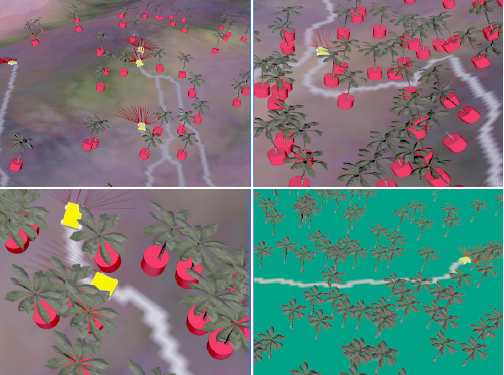
\includegraphics[width=0.33\textwidth,height=5cm]{images/robombeiros2.png}
	    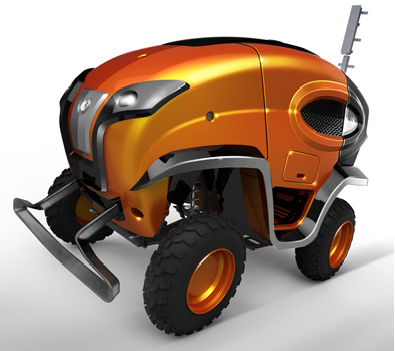
\includegraphics[width=0.33\textwidth,height=5cm]{images/jacto.png}
	    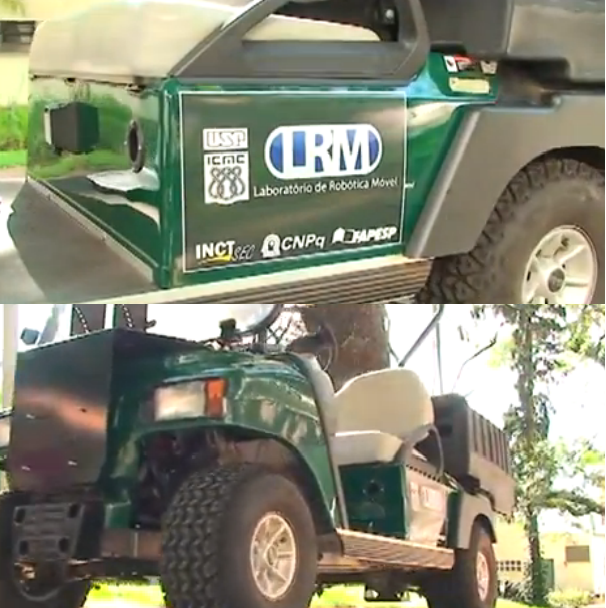
\includegraphics[width=0.33\textwidth,height=5cm]{images/carina_1_stacked.png}
	 	\caption{Simulador RoBombeiros (\textit{esquerda}), 
	 	Jacto JAV (\textit{centro}), CaRINA I (\textit{direita})}
		\fonte{(Jacto S/A, LRM–ICMC/USP)}
	 	\label{fig:um}
 	\end{minipage}
\end{figure}

%2012-10-15 Lido OK


% \section{Contribuições Esperadas}

As principais contribuições acadêmico-científicas esperadas deste trabalho são: 

\begin{enumerate}[i.]

\item adaptação e aperfeiçoamento dos algoritmos para a geração em “tempo real”
de mapas de disparidade, obtendo estes mapas a partir de um par de imagens
capturadas pela câmera estéreo;

\item proposta e desenvolvimento de algoritmos para a obtenção de mapas locais
de navegabilidade com informações espaciais (3D), onde o espaço tridimensional
será dividido em regiões e estas regiões serão identificadas como sendo
navegáveis ou não navegáveis;

\item aperfeiçoamento de técnicas para a navegação baseada no uso de GPS,
bússola e mapas locais de navegabilidade, onde as pesquisas previamente
desenvolvidas para detectar e desviar de obstáculos com o uso de mapas 2D, serão
estendidas a fim de trabalhar com mapa de navegabilidade/ocupação em 3D. Deste
trabalho resultará um sistema com possibilidade de aplicação prática em
importantes tarefas de navegação autônoma, como por exemplo, em sistemas
voltados para aplicações agrícolas e em sistema de combate a incêndio em
florestas, tarefas estas que podem ser perigosas para o ser humano (por exemplo,
exposição prolongada aos produtos químicos de defensivos agrícolas, e
combate/contato direto com fumaça e incêndios).

\end{enumerate}

% \section{Objetivo Geral}
\label{sec:obj_geral}

O objetivo geral deste trabalho é desenvolver um sistema de navegação autônoma baseado
em visão computacional a fim de capacitar um veículo terrestre autônomo a se locomover em
ambientes externos não estruturados, ou seja, em campos com vegetação/plantação e/ou em
florestas pouco densas. O veículo deverá ser capaz de se dirigir até uma localização determinada,
desviando dos obstáculos, percebendo-os de forma autônoma, e escolhendo por meios próprios o
caminho a seguir. O veículo autônomo deverá ter a capacidade de identificar os elementos do terreno
onde irá se deslocar, identificando o chão e os obstáculos, a fim de evitar zonas não transponíveis ou
muito acidentadas. Portanto, o objetivo deste trabalho é desenvolver um sistema de navegação
robusto e seguro voltado à aplicação em veículos autônomos para ambientes externos não
estruturados (ou muito pouco estruturados), baseado no uso de visão computacional realizada
através da captura de imagens estéreo, no uso de mapas de profundidade (mapas de disparidade), e
no uso mapas locais de navegabilidade.

%2010-10-10 REVISAR


%%%\section{Objetivo e Hipótese}

O objetivo deste trabalho é desenvolver um sistema de navegação autônoma baseado
em visão computacional a fim de capacitar um veículo terrestre a se locomover em
ambientes externos não estruturados, ou seja, um campo com vegetação/plantação
e/ou floresta pouco densa. O veículo deverá ser capaz de desviar de obstáculos,
percebendo-os de forma autônoma, e se dirigir até uma localização determinada
escolhendo por meios próprios o caminho a seguir. Deverá ter alguma capacidade
de reconhecer o terreno que irá se deslocar a fim de evitar zonas não
transponíveis ou muito acidentadas.

A informação espacial tridimensional representa mais precisamente o ambiente
onde o veículo autônomo se encontra e por onde deve se locomover, portanto, os
métodos de navegação e representação do ambiente baseados nesta informação
tridimensional são mais abrangentes e menos limitados em relação ao controle e
conhecimento do ambiente.

Tem-se por hipótese então, que algoritmos de navegação planares podem ser
expandidos para o espaço tridimensional se tornando menos limitados e mais
robustos.

%2012-10-15 Revisar

\section{Objetivos Específicos}

Os principais objetivos específicos deste projeto de mestrado, que se apresentam
como um desdobramento do objetivo geral descrito acima, são:

\begin{itemize}

\item Extração de referenciais a partir de um par de câmeras, constituindo um
sistema de visão binocular (estéreo);

\item Propor melhorias nos algoritmos de geração do mapa de disparidade, obtido
a partir das imagens estéreo;

\item Gerar um mapa de navegabilidade local a partir de informações visuais;
%,
%que possa ser adaptado a algoritmos de planejamento e controle de navegação
%autônoma;

\item Desenvolver um mecanismo de navegação autônoma, baseado nas informações de
GPS, Bússola e do Sistema de Visão, capaz de desviar de obstáculos e dirigir o
veículo até um destino determinado de forma robusta e eficiente;

\item Fazer uso dos conhecimentos prévios de trabalhos desenvolvidos no
laboratório e contribuir para a consolidação de tecnologias capazes de atribuir
navegabilidade autônoma a veículos de diversas naturezas para fins práticos;

\item Aplicação e avaliação do sistema de navegação autônoma em um veículo real
em ambiente externo não estruturado.

\end{itemize}

%2012-10-15 Revisar
